\documentclass{standalone}
\usepackage{tikz}
\begin{document}
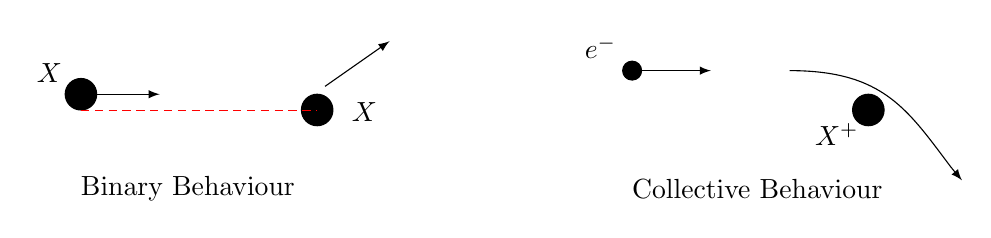
\begin{tikzpicture}
    \node [label={[shift={(0.6,-0.4)}] $X$}] (A) at (0,0) {};
    \node [label={[shift={(-0.4,-0.1)}] $X$}] (B) at (-3,0.20) {};
    \draw[black,fill=black] (B) circle (0.2);
    \draw[black,fill=black] (A) circle (0.2);
    \draw[-latex] (B) -- +(0:1); % Velocity arrow
    \draw[-latex] (0.1,0.3) -- +(35:1); % New velocity arrow
    \draw[red,line width=0.2pt, densely dashed] (-3,0.0) -- (0,0.0);
    \node[text width=3cm] at (-1.5,-1) {Binary Behaviour}; % Text node
    % End of binary collision
    % Start of collective collision
    \node [label={[shift={(-0.4,-0.7)}] $X^+$}] at (7,0) {};
    \node [label={[shift={(-0.4,-0.1)}] $e^-$}] at (4,0.5) {};
    \draw[black,fill=black] (4,0.5) circle (0.12);
    \draw[black,fill=black] ([shift=({7,0})]A) circle (0.2);
    \draw[-latex] (4,0.5) -- +(0:1); % Velocity arrow
    \draw[-latex] (8.06,-0.74) -- +(-50:0.2); % New velocity arrow
    \draw (6,0.5) .. controls (7.2,0.5) and (7.5,-0.0) .. (8.06,-0.74);
    \node[text width=4cm] at (6,-1) {Collective Behaviour}; % Text node
\end{tikzpicture}
\end{document}